\documentclass[xelatex,ja=standard]{bxjsarticle}
\usepackage[utf8]{inputenc}
\usepackage{amsmath}
\usepackage{amsfonts}
\usepackage{amssymb}
\usepackage{tabularx}
\usepackage{booktabs,dcolumn}
\usepackage{bbm}
\usepackage{natbib}
\setlength{\bibsep}{0.0pt}
\usepackage{graphicx}
\usepackage{setspace}
\usepackage{geometry}
\usepackage{array}
\usepackage[labelformat=simple]{subcaption}
\usepackage{setspace}
\usepackage[titletoc]{appendix}
\usepackage{changepage}
\usepackage{footmisc}
\usepackage{authblk}
\usepackage[disable, colorinlistoftodos,backgroundcolor=white, bordercolor=red, textcolor=red, textsize=tiny]{todonotes}
\usepackage{pdfpages}
\usepackage{subcaption}
\usepackage{comment}
%\usepackage{url} % 文献でのURL表示

\usepackage{lscape}
\usepackage{pdflscape}
\usepackage{rotating}

\usepackage{color}
\definecolor{MyBlue}{rgb}{0,0,0.6}
\usepackage[bookmarks=true,%
bookmarksnumbered=true,%
colorlinks=true,%
linkcolor=MyBlue,%
citecolor=MyBlue,%
filecolor=MyBlue,%
urlcolor=MyBlue%
]{hyperref}

\onehalfspacing
\bibpunct{(}{)}{;}{a}{}{;}
\geometry{top=2cm, bottom=2cm, left=3cm, right=3cm}
\newcolumntype{Z}{>{\centering\arraybackslash}X}
\abovecaptionskip=-2pt
\setlength{\marginparwidth}{2cm} % for todonotes
\usepackage{fontspec}
\usepackage{underscore}
\usepackage[T1]{fontenc}
  
\setCJKsansfont[Path = ../../../\detokenize{01_admin}/preamble/tex/fonts/,
BoldFont = HaranoAjiGothic-Bold.otf]
{HaranoAjiGothic-Regular.otf}

\setCJKmainfont[Path = ../../../\detokenize{01_admin}/preamble/tex/fonts/,
BoldFont = HaranoAjiMincho-Bold.otf]
{HaranoAjiMincho-Regular.otf}

\usepackage{threeparttable}
\usepackage{float}

\title{朝ごはんと成績に統計的関係があるか \\ -- Peanutsのデータを用いて -- \thanks{本レポートは、データサイエンスの授業において、R/RStudio、Git/GitHub、LaTeX/Overleafを組み合わせて、再生可能なプログラミングと文書作成の例として作成したものである。レポートの書式としては、あくまで内部資料として作成しており、外部向けの論文の形式を取っていない。また、Peanutsの設定は全て仮想である。}}

\author{Charlie Schultz
\thanks{Department of Comics. Email: cshultz@comics.edu}  \ \  Chishio Furukawa
\textsuperscript\thanks{Department of Economics. Email:cfurukawa@economics.ac.jp}}

%\date{\today}
\date{March, 1990}


\begin{document}
\renewcommand\footnotelayout{\small}
\sffamily\mdseries

\maketitle

\vspace{-10pt}\begin{abstract}
\begin{spacing}{1}
\noindent 
Peanutsの登場キャラクターたちは、自分たちの経験に基づき「好きな朝ごはんを食べることが、学校の成績につながる」と考えています。本レポートでは、この統計的根拠を探索し、以下の結果を得ました。(1)朝ごはんに``pancake''を食べることは、小テストの成績と強く相関はしていなかった。(2)Snoopyが``corn flake''の代わりに``dog flake''ばかり買ったときには「朝ごはんに``dog flake''を食べ、アレルギーで勉強に集中できなかった」とCharlieとSallyは言っていますが、これについては整合的な根拠が示された。\\

\end{spacing}
\end{abstract}

\newpage

\section{はじめに}

\subsection{背景} 

この統計分析は、朝ごはんと成績の関係性を吟味することを目的としている。CharlieやLucieらは、「おいしい朝ごはんを食べることが学校の成績に欠かせない」と信じている。特に、pancakes(和製英語:ホットケーキ)は好物で、トーストやオートミールよりも、pancakesをもっと食べたいと考えている。学術的にも、朝ごはんを食べることが学校の成績と相関していると言われている()。

\subsection{問い}

本レポートでは、James Elementary Schoolと、それぞれの朝ごはんの記録のデータを結び付けて、次の2つの問いについて考える。

\begin{enumerate}
\item pancakeを食べることは、学校の成績に相関しているだろうか。
\item 「dog flakesを食べることによって、勉強に集中できず、成績が悪くなった」という主張は、統計的に整合的だろうか。
\end{enumerate}

\subsection{記述統計}

まず、統計分析をはじめる前に、登場キャラクターが、どのような朝ごはんを食べているかをまとめよう。

\begin{table}[!h]
\centering
\begin{tabular}[t]{lrr}
\toprule
breakfast\_renamed & count & frequency\\
\midrule
cereal & 292 & 0.33\\
dog flakes & 6 & 0.01\\
no breakfast & 41 & 0.05\\
oatmeal & 206 & 0.23\\
pancakes & 178 & 0.20\\
\addlinespace
toast & 172 & 0.19\\
\bottomrule
\end{tabular}
\end{table}


\begin{itemize}
\item もっともよく食べるものは、cerealやtoastなどである。
\item pancakeを食べることは稀であり、特別だということが分かる。
\item dog flakesを食べなくてはいけないことは数回しかなかった。
\end{itemize}

\section{分析} 



\begin{figure}
\centering
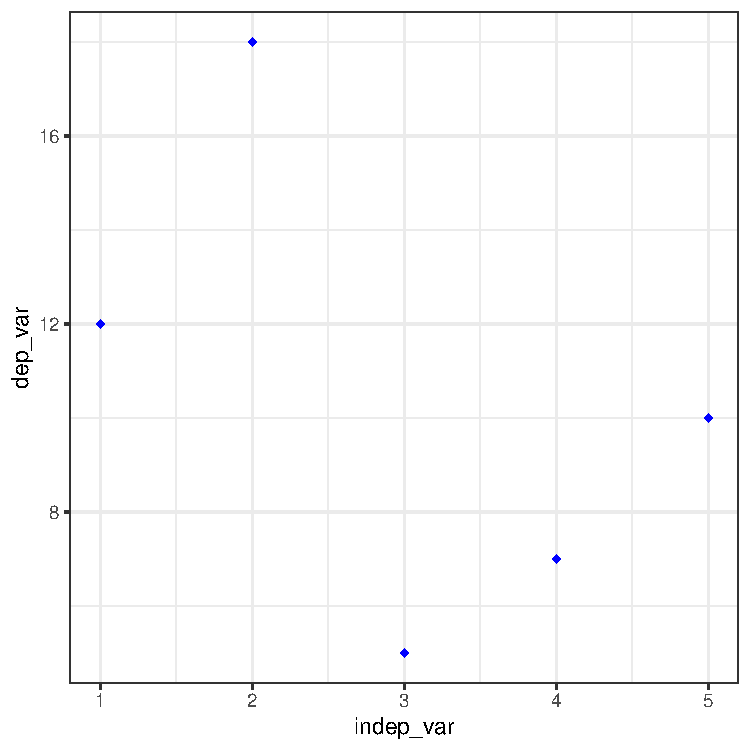
\includegraphics[width=7cm]{04_analyze/scatter_regress/figure/figure.pdf}

\label{fig:img1}
\caption{Bare figure}
\end{figure}

\mcfamily\mdseries

\begin{table}

\caption{Initial regressions}
\centering
\begin{threeparttable}
\begin{tabular}[t]{lcc}
\toprule
\multicolumn{1}{c}{ } & \multicolumn{1}{c}{(1)} & \multicolumn{1}{c}{(2)} \\
\cmidrule(l{3pt}r{3pt}){2-2} \cmidrule(l{3pt}r{3pt}){3-3}
  & Average & Average \\
\midrule
freq(pancakes) & 2.42 & 2.19\\
 & (2.07) & (2.03)\\
Constant & 44.39 & \\
 & (3.15) & \\
\midrule
Num.Obs. & 111 & 111\\
R2 & 0.033 & 0.072\\
Model & OLS & FE\\
NA & NA & NA\\
Clustering & Y & Y\\
R2 Adj. & 0.024 & 0.046\\
\bottomrule
\end{tabular}
\begin{tablenotes}
\item \textit{Note: } 
\item Heteroskedasticity-robust standard errors clustered at students level are reported in the parenthesis.
\end{tablenotes}
\end{threeparttable}
\end{table}



Peanutsの登場キャラクターたちは、自分たちの経験に基づき「好きな朝ごはんを食べることが、学校の成績につながる」と考えています。本レポートでは、この統計的根拠を探索し、以下の結果を得ました。(1)朝ごはんに``pancake''を食べることは、小テストの成績と強く相関はしていなかった。(2)Snoopyが``corn flake''の代わりに``dog flake''ばかり買ったときには「朝ごはんに``dog flake''を食べ、アレルギーで勉強に集中できなかった」とCharlieとSallyは言っていますが、これについては整合的な根拠が示された。


\bibliographystyle{econ} 
\bibliography{01_admin/preamble/tex/literature.bib}

\end{document}